\section{Results}\label{sec:mvtraits-results}

\subsection{Estimates of PFT-level means}

\begin{figure}
  \centering
  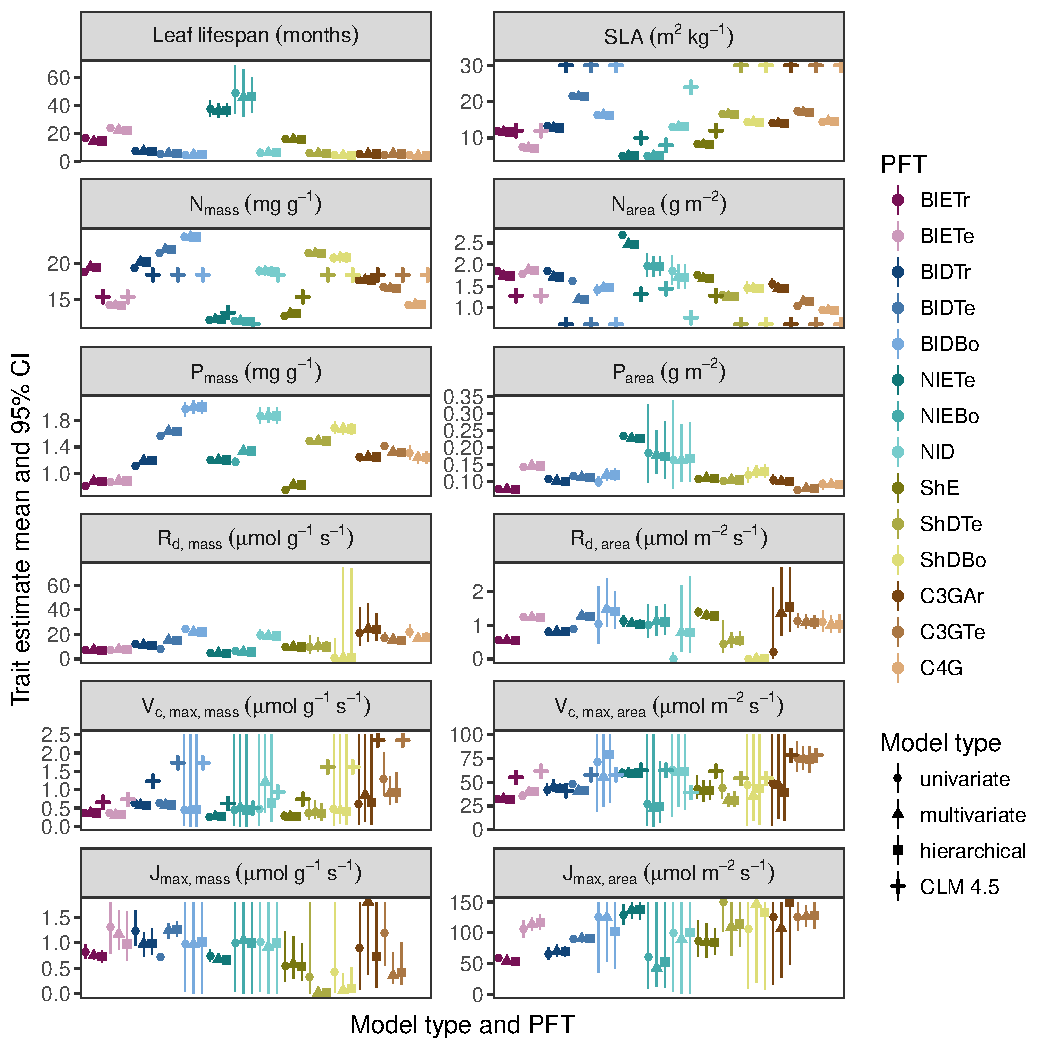
\includegraphics[width=\textwidth]{1_mvtraits/figures/mean_comparison.pdf}
  \caption{%
    Mean and 95\% confidence interval on best estimates of traits for each plant functional type from the univariate, multivariate, and hierarchical models.
    For leaf lifespan and SLA, results were not significantly different between the mass- and area-based models, so only results from the mass-based model are shown.
    For some PFT-trait combinations, where large error bars resulting from the relatively uninformative priors are substantially larger than the variability among means, the $y$ axes are constrained to facilitate comparison.
  }\label{fig:mvtraits-fig2}
\end{figure}

In general, leaf trait estimates from the univariate, multivariate, and hierarchical models were similar (Fig.~\ref{fig:mvtraits-fig2}).
Where we observed differences between models, the largest were between the univariate and multivariate models, while the additional constraint from the hierarchical model tended to have a minimal effect on trait estimates.
Significant differences in trait estimates between univariate and multivariate models occurred even for traits with relatively large sample sizes, such as leaf nitrogen content.

Evergreen PFTs had by far the largest leaf lifespan, with the longest lifespan observed for temperate and boreal needleleaf evergreen species.
Meanwhile, all of deciduous species had lifespans shorter than 7 months.
Among deciduous species, lifespan was generally longer in warmer biomes than colder ones.

Across-PFT patterns in SLA and $N_{\mass}$, $P_{\mass}$, and $R_{d,\mass}$ were similar.
Temperate broadleaved deciduous trees and shrubs generally had among the highest values of these traits, while temperate evergreen trees and shrubs had generally among the lowest.
However, none of these patterns were universal to all four traits.
For example, tropical evergreen trees had relatively high $N_{\mass}$ and mean SLA and $R_{d,\mass}$, but among the lowest $P_{\mass}$.
Similarly, temperate and boreal shrubs had higher $N_{\mass}$ and $P_{\mass}$ than any of the grasses, but comparable SLA\@.

Across-PFT patterns in $N_{\area}$, $P_{\area}$, and $R_{d,\area}$ were different from their mass-normalized counterparts.
For example, tropical broadleaved evergreen and needleleaf evergreen trees had among the lowest $N_{\mass}$ and $P_{\mass}$ basis but among the highest $N_{\area}$ and $P_{\area}$, while the opposite was true of deciduous temperate trees and shrubs.
Species with N contents near the middle of the observed range did not shift as dramatically depending on type of normalization.

C3 grasses had both the highest $V_{c,\max,\mass}$ and $V_{c,\max,\area}$.
Compared to broadleaved trees, temperate needleleaved evergreen trees had lower $V_{c,\max,\mass}$ but higher $V_{c,\max,\area}$.
Among broadleaved trees, deciduous trees had higher $V_{c,\max,\mass}$ and slightly higher $V_{c,\max,\area}$ than evergreen trees.
Between the deciduous and evergreen tree PFTs, we observed no significant trend by climate zone.

C3 grasses and temperate needleleaved evergreen trees had the highest $J_{\max,\area}$, but temperate broadleaved deciduous trees had the highest $J_{\max,\mass}$.
All of the shrub PFTs had the lowest $J_{\max,\mass}$ but average or above-average $J_{\max,\area}$, while the opposite was true of broadleaved tropical PFTs.
Of the tree PFTs, needleleaved evergreen trees had the highest $J_{\max,\area}$ but the lowest $J_{\max,\mass}$.

A key application of this study was to provide data-driven parameter estimates for Earth System Models.
To this end, we compared our mean parameter estimates with corresponding default parameters in CLM 4.5~\cite{clm45_note} (Fig.~\ref{fig:mvtraits-fig2}).
Our mean estimates of SLA agreed with CLM's defaults~\cite[Table 8.1 in]{clm45_note} only for tropical broadleaved evergreen trees, and for all other PFTs, our estimates are significantly lower.
For $N_{\mass}$, our estimates agreed reasonably well with CLM for evergreen temperate trees, needleleaved trees, and C3 arctic grasses, and were substantially different for all other PFTs.
Our $N_{\mass}$ estimates also varied much more across PFTs than CLM's parameters.
For $N_{\area}$, our estimates were significantly higher than CLM's for all PFTs, likely due to CLM's overestimates of SLA\@.
Our estimates of $V_{c,\max_\mass}$ were lower across all PFTs, with particularly large differences for tropical and temeprate broadleaf deciduous trees and evergreen shrubs, and temperate C3 grasses.
Our estimates of $V_{c,\max,\area}$ showed better agreement, though our values were still significantly lower for many PFTs.
Like us, Kattge et al.~(2009) \nocite{kattge_2009_vcmax} also found that $V_{c,\max,\area}$ was overestimated by Earth System models,
but their estimates of $V_{c,\max,\area}$ and $N_{\area}$ are generally slightly higher than ours.

\begin{figure}
  \centering
  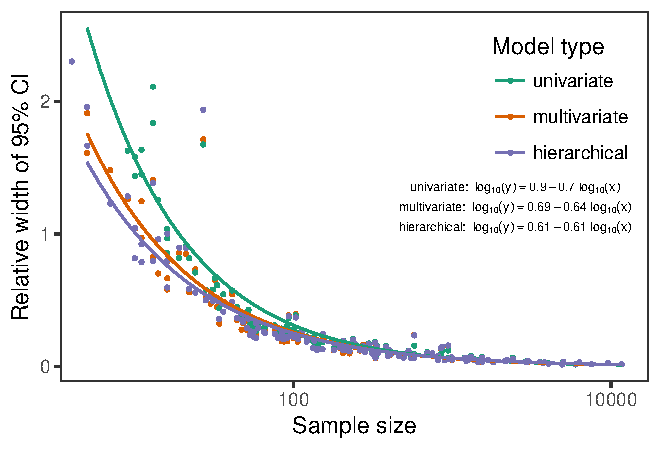
\includegraphics[width=\textwidth]{1_mvtraits/figures/relative_ci_model.pdf}
  \caption{%
    Relative uncertainty in PFT-level trait estimates as a function of sample size for each model type.
    Lines represent linear models ($\log(y) = b_0 + b_1 \log(x)$) fit independently for each model type.
    In general, differences in estimate uncertainty between the univariate and multivariate models were minimal at large sample sizes but increasingly important at low sample sizes.
    However, differences in estimate uncertainty between the multivariate and hierarchical models were consistently negligible.
  }\label{fig:mvtraits-fig3}
\end{figure}

We observed clear differences in the relative uncertainties of mean estimates with respect to sample size.
All of the high-latitude PFTs consistently had among the largest error bars around their mean estimates relative to other PFTs, while the traits with the largest uncertainties were dark respiration, $V_{c,\max}$, and $J_{\max}$.
For many of these trait-PFT combinations, the additional constraint from trait covariance provided by the multivariate and hierarchical models substantially reduced error bars, making it possible to compare estimates against those of other PFTs.
Our analysis of the relationship between model type, sample size, and estimate relative uncertainty found that this covariance-based constraint from the multivariate model both reduced uncertainty overall (lower intercept) and reduced the sensitivity of estimate uncertainty to sample size (lower slope) compared to the univariate model (Fig.~\ref{fig:mvtraits-fig3}).
However, this analysis revealed no consistent significant benefit from the hierarchical model.


\subsection{Trait correlation patterns across- and within-PFTs}

\begin{figure}
  \centering
  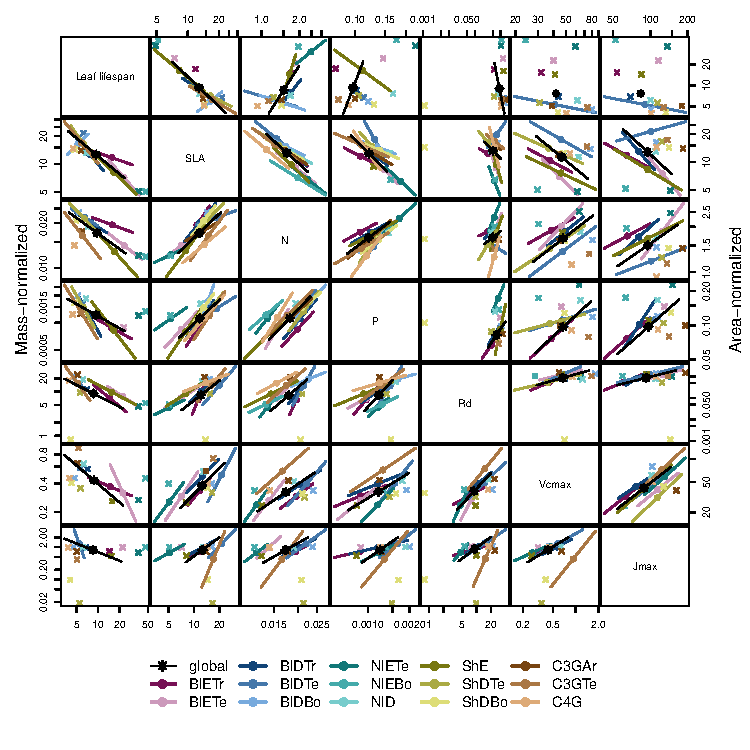
\includegraphics[width=\textwidth]{1_mvtraits/figures/stick_pairs.pdf}
  \caption{%
    Pairwise trait mean and covariance estimates for all data pooled globally (black) and for each PFT (colored).
    Covariance estimates not significantly different from zero ($p < 0.05$) are indicated by x symbols at the mean estimate.
    $x$ and $y$ axes vary on a log scale, reflecting the fact that the model was fit using the base 10 log of all traits.
    With the exception of leaf lifespan, pairwise covariances are consistent in direction but vary somewhat in magnitude between PFTs, and when comparing PFT-level and global estimates.
    However, many pairwise covariances are not statistically significant, particularly (but not always) for undersampled traits and PFTs.
  }\label{fig:mvtraits-fig4}
\end{figure}

For all traits except leaf lifespan, pairwise trait correlations were generally consistent in direction both globally and within each PFT (Fig.~\ref{fig:mvtraits-fig4}).
In particular, mass- and area-normalized traits were all positively correlated with each other and, respectively, positively and negatively correlated with SLA, both globally and within each PFT\@.
The same was generally true of correlations of mass-based traits with leaf lifespan, but correlations of leaf lifespan with area-normalized traits were more variable.
The correlation between $N_{\area}$ and leaf lifespan was positive globally and for evergreen shrubs, tropical broadleaved deciduous trees, temperate needleleaved evergreen trees but negative for temperate and boreal broadleaved deciduous trees and not significant for any other PFTs.
Similarly, the correlation between $P_{\area}$ and leaf lifespan was positive globally but negative for evergreen shrubs and not significant for any other PFTs.
The correlation between leaf lifespan and $R_{d,\area}$ was significant and negative globally, but was not significant within any PFTs.
The only significant correlations of leaf lifespan with $V_{c,\max,\area}$ and $J_{\max,\area}$ were negative for temperate broadleaved deciduous trees.

A large number of pairwise trait correlations were not significant.
In some cases, this was driven by sample size (Fig.~\ref{fig:mvtraits-fig1}).
For instance, needleleaved deciduous trees, the most undersampled PFT in our analysis, were often the only PFT for which a correlation was not statistically significant.
In other cases, though, PFTs with smaller sample sizes had significant pairwise correlations while PFTs with much larger sample sizes had none.
For example, tropical broadleaved evergreen trees were relatively well-sampled for all traits, but none of their area-normalized traits were significantly correlated with leaf lifespan.
In general, we observed fewer significant trait correlations among area-normalized traits than mass-normalized traits. 

\begin{figure}
  \centering
  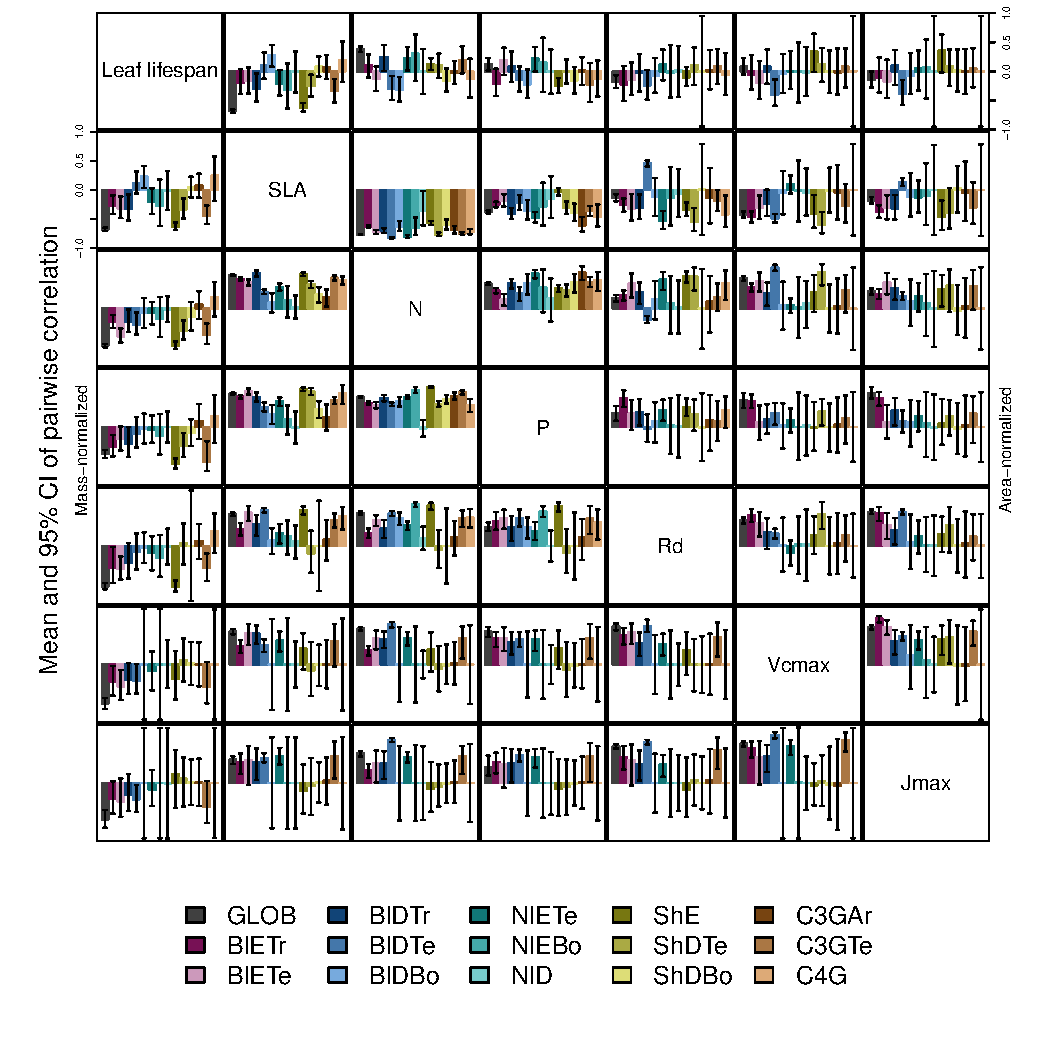
\includegraphics[width=\textwidth]{1_mvtraits/figures/correlation_boxplot.pdf}
  \caption{%
    Mean and 95\% CI on estimates of pairwise correlation coefficients
    for all data pooled globally (dark grey) and for each PFT (colored).
    For most PFT-trait pairs, correlations are mutually consistent in magnitude but vary in strength.
  }\label{fig:mvtraits-fig5}
\end{figure}

The strength of pairwise trait correlations varied substantially depending on scale, PFT, and trait (Fig.~\ref{fig:mvtraits-fig5}).
The two pairwise trait correlations that exhibited the most consistent strength globally and within each PFT were the correlation between SLA and $N_{\area}$, and between $N_{\mass}$ and $P_{\mass}$.
Correlation strength was often, but not always, related to sample size, with well-sampled PFTs exhibiting stronger correlations and undersampled PFTs exhibiting weaker correlations.
